\documentclass[10pt]{article}

\usepackage[margin=0.75in]{geometry}
\usepackage{amsmath,amsthm,amssymb}
\usepackage{xcolor}
\usepackage{cancel}
\usepackage{graphicx}
\usepackage{changepage}
\usepackage{tikz}
\usepackage{pgfplots}
\usepackage{physics}
\usepackage{minted}
\usepackage{hyperref}
\usepackage[breakable]{tcolorbox}
\usepackage[inline]{enumitem}

\theoremstyle{definition}
\newtheorem{problem}{Problem}
\newtheorem{soln}{Solution}

\pgfplotsset{compat=newest}
\usetikzlibrary{lindenmayersystems}
\usetikzlibrary{arrows}

\definecolor{incolor}{HTML}{303F9F}
\definecolor{outcolor}{HTML}{D84315}
\definecolor{cellborder}{HTML}{CFCFCF}
\definecolor{cellbackground}{HTML}{F7F7F7}

\tikzset
{%
  axes/.style={thick,-latex},
  cylinder/.style={right color=blue!80,left color=white,fill opacity=0.7},
  paraboloid back/.style={left color=magenta!80,fill opacity=0.4},
  paraboloid front/.style={left color=white, right color=magenta!80,fill opacity=0.4},
}

\makeatletter
\newcommand{\boxspacing}{\kern\kvtcb@left@rule\kern\kvtcb@boxsep}
\makeatother
\newcommand{\prompt}[4]{
    \ttfamily\llap{{\color{#2}[#3]:\hspace{3pt}#4}}\vspace{-\baselineskip}
}


\hypersetup{
    colorlinks=true,
    linkcolor=blue,
    filecolor=magenta,      
    urlcolor=cyan,
    pdftitle={Overleaf Example},
    pdfpagemode=FullScreen,
    }

\NewDocumentCommand{\evalat}{sO{\big}mm}{%
  \IfBooleanTF{#1}
   {\mleft. #3 \mright|_{#4}}
   {#3#2|_{#4}}%
}

\tikzset{koch snowflake/.style={insert path={%
   l-system [l-system={rule set={F -> F-F++F-F}, axiom=F++F++F,
    step=3cm/3^#1, angle=60, order=#1,anchor=center}] -- cycle}}}

\title{Physics II: Lab 4}
\author{Jeremy Favro}
\date{\today}

\begin{document}

\maketitle

\noindent Experiment performed on station \#2 with labelled radius of curvature $R=42\pm 1$cm.

% PROBLEM 1
\begin{problem}
Plot $r_m^2$ (on the vertical axis) versus $m$ (horizontal axis) using a spreadsheet. Label both axes with appropriate units if applicable. Add a linear trendline
to the graph as we expect a linear relationship between the variables.
\end{problem}
\begin{soln} ~\\
  \begin{center}
    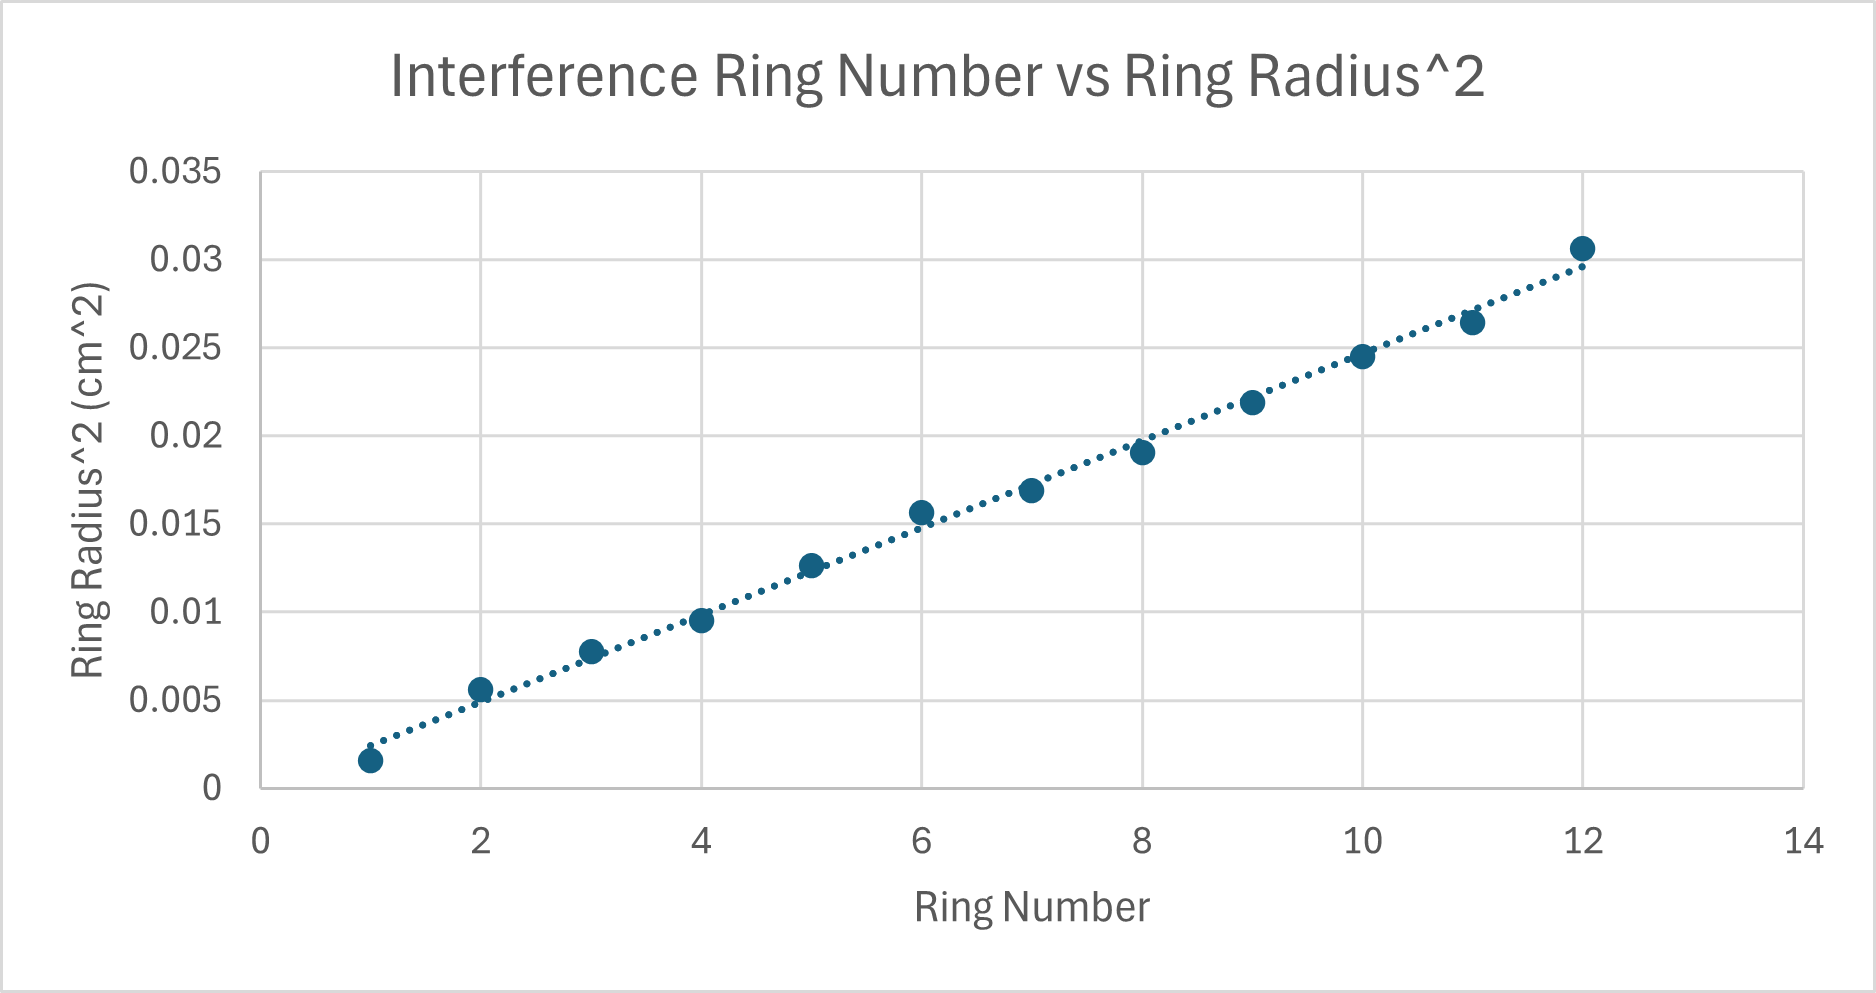
\includegraphics{Picture1.png}
  \end{center}
\end{soln}

% PROBLEM 2
\begin{problem}
Compute the slope of the graph and its associated uncertainty using LINEST or another similar method. Report both including units.
\end{problem}
\begin{soln}
  Using LINEST in Microsoft Excel I calculated the slope to be $0.00246843\pm3.41288\cdot 10^{-5} \text{cm}^2$
\end{soln}

% PROBLEM 3
\begin{problem}
Find the wavelength of light $\lambda$ from the slope and using your station's labeled radius of curvature $R$.
Do the same calculation on the uncertainty in the slope to find the uncertainty in the wavelength, $\delta\lambda$.
\end{problem}
\begin{soln}
  We were given $R=42 \pm 1 \text{cm}$. Calculating $\lambda$:
  \begin{align*}
     & \lambda R = 0.00246843\pm3.41288\cdot 10^-5 \\
     & \lambda = \frac{0.00246843}{R}              \\
     & \lambda = 5.87721\cdot 10^{-5}              \\
     & \lambda = 5.87721 \text{cm}                 \\
  \end{align*}
  And $\delta\lambda$:
  \begin{align*}
     & \delta\lambda R = 3.41288\cdot 10^-5             \\
     & \delta\lambda = \frac{3.41288\cdot 10^-5 }{R}    \\
     & \delta\lambda = 8.324095 \cdot 10^{-7} \text{cm} \\
  \end{align*}
  $\therefore \lambda = (5.877 \pm .083)\cdot 10^{-5}\text{cm}$
\end{soln}


% PROBLEM 4
\begin{problem}
Which wavelength did you observe? Does the wavelength that you calculated agree with any of these values within uncertainty? Comment briefly and show any calculations.
\end{problem}
\begin{soln}
  The maximum and minimum bounds for $\lambda$ are $\lambda_{max}=5.960\cdot10^{-5}$cm and $\lambda_{min}=5.790\cdot10^{-5}$cm which fits the wavelength of the sodium lamp best
  as $\lambda_{sodium}=5.890\cdot 10^{-5}$cm which sits comfortably in the middle of the range of possible values as shown below

  \begin{tikzpicture}[scale=8]
    \draw[<->] (4,0) -- (6,0) ;
    \foreach \x in  {4.358,5.461,5.770,5.791,5.890}
    \draw[shift={(\x,0)},color=black] (0pt,0.5pt) -- (0pt,-0.5pt);
    \foreach \x in {4.358,5.770}
    \draw[shift={(\x,0)},color=black] (0pt,0pt) -- (0pt,-3pt) node[below] {$\x\cdot10^{-5}$cm};
    \foreach \x in {5.461,5.791}
    \draw[shift={(\x,0)},color=black] (0pt,0pt) -- (0pt,3pt) node[right, rotate=90] {$\x\cdot10^{-5}$cm};

    \draw[shift={(5.890,0)},color=blue] (0pt,0pt) -- (0pt,3pt) node[right, rotate=90] {$5.890\cdot10^{-5}$cm};


    \draw[*-*, blue] (5.79,0) -- (5.96,0);
    \draw[very thick, blue] (5.79,0) -- (5.96,0);
  \end{tikzpicture}
\end{soln}

% PROBLEM 2
\begin{problem}
What are sources of error that contribute to the uncertainty in the calculate wavelength? Can you think of plausible ways to decrease this uncertainty by modifying the experiment procedure?
Comment briefly on both questions.
\end{problem}
\begin{soln}
  A relatively significant source of error that myself and my group encountered was different readings by different people on the Vernier scale. Generally we agreed
  but occasionally different measurements were observed by different people. The difference was very minor, but still likely a contributor to the error present. A digital method of measuring ring
  diameter would likely help alleviate measurement uncertainty as a source of potential error. Other than that the setup was quite dusty, which may have very slightly affected the results observed,
  however I imagine the effects from that would be very minor. Dusting off the apparatus before performing the experiment may have decreased the error very slightly.
\end{soln}
\end{document}